%!TEX root = ../thesis-guntur.tex
%********************************************************************
% Appendix - ambient noise recordings
%*******************************************************
% If problems with the headers: get headings in appendix etc. right
%\markboth{\spacedlowsmallcaps{Appendix}}{\spacedlowsmallcaps{Appendix}}
\chapter{Ambient Noise Recordings}
\label{ch:appendix-ambient-noise}

\section{Day 1} % (fold)
\label{sec:ambient-noise-day_1}
\begin{figure}[H]
	\centering
	\subfloat[peak level]{
		\label{fig:peak-level-day1}{
			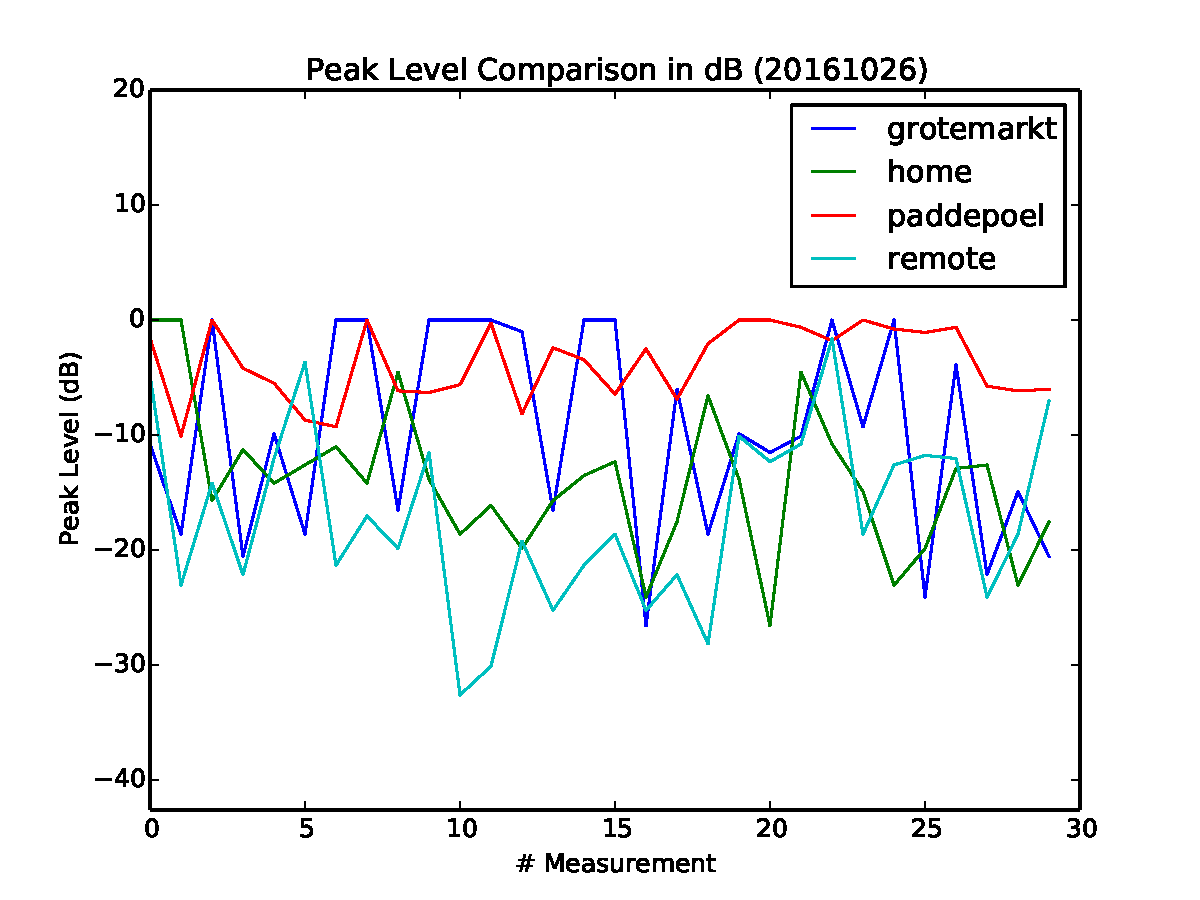
\includegraphics[width=0.7\textwidth]{./img/result/sound/peak-level-comparison-20161026}
		}
	}
	\subfloat[root mean square]{
		\label{fig:rms-day1}{
			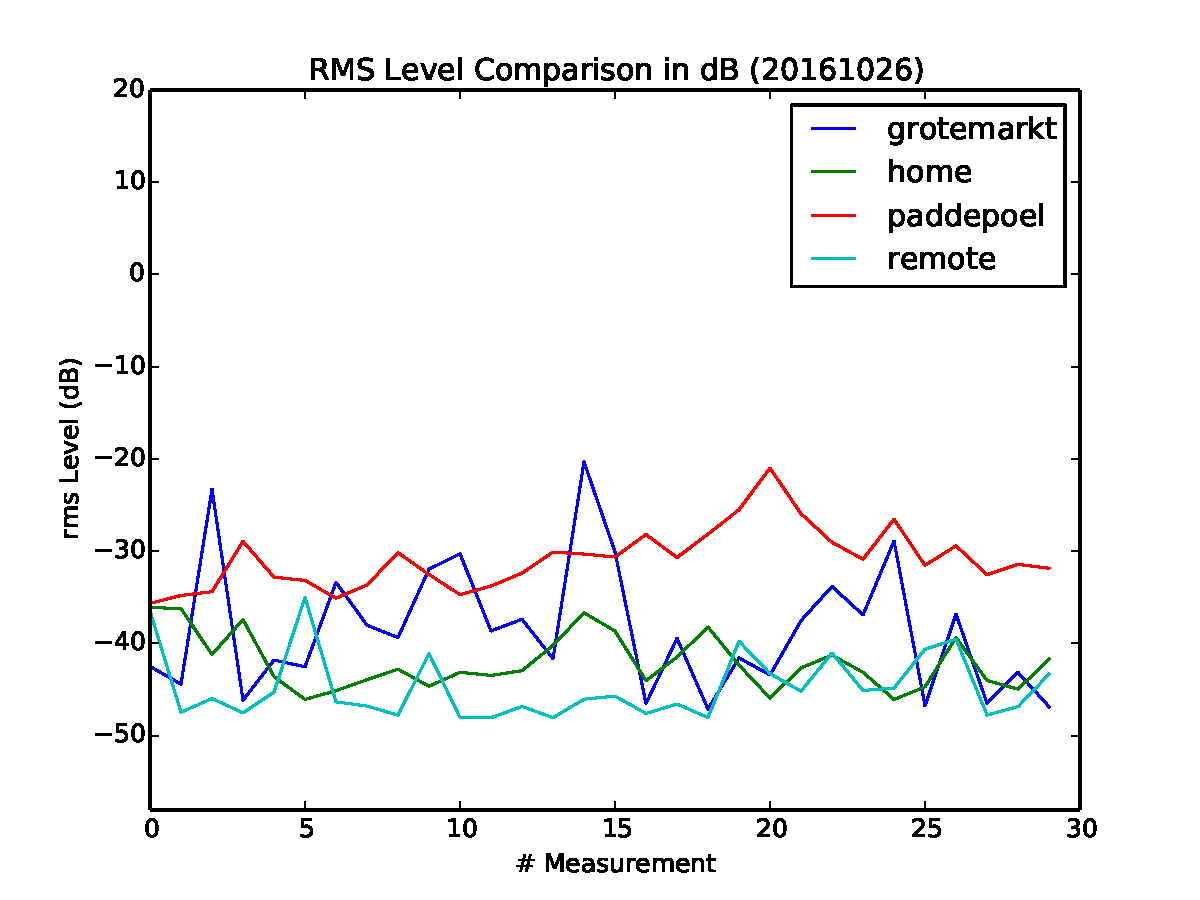
\includegraphics[width=0.7\textwidth]{./img/result/sound/rms-level-comparison20161026}
		}
	}
	\caption{Line chart showing the peak level (\ref{fig:peak-level-day1}) and root-mean-square (\ref{fig:rms-day1}) in each cycle at day 1.}
	\label{fig:audio-result-day1}
\end{figure}

\begin{table}[H]
\centering
\caption{The average of root-mean-square and peak level of ambient noise recording in day 1.}
\label{tab:ambient-noise-average-day1}
\begin{tabular}{lll} \toprule
            & \ac{RMS} (dB) & \ac{PKLV} (dB) \\ \midrule
Remote area & -44.74                & -17.06          \\
Home        & -42.07                & -14.04           \\
Paddepoel   & -30.86                & -3.74          \\
Grote markt & -38.57              & -9.67        \\ \bottomrule
\end{tabular}
\end{table}




\section{Day 2} % (fold)
\label{sec:ambient-noise-day_2}
\begin{figure}[H]
	\begin{adjustwidth}{-4cm}{}
	\centering
	\subfloat[peak level]{
		\label{fig:peak-level-day2}{
			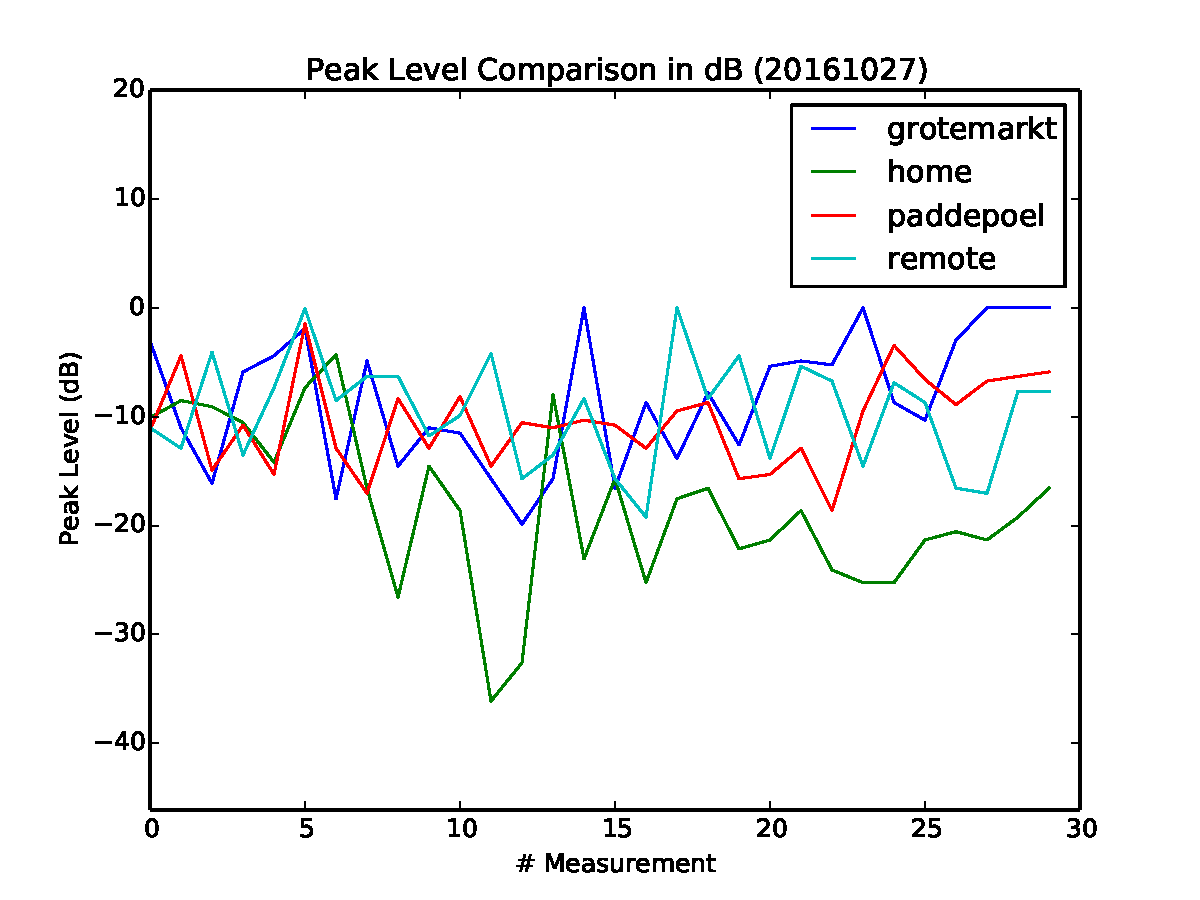
\includegraphics[width=0.7\textwidth]{./img/result/sound/peak-level-comparison-20161027}
		}
	}
	\subfloat[root mean square]{
		\label{fig:rms-day2}{
			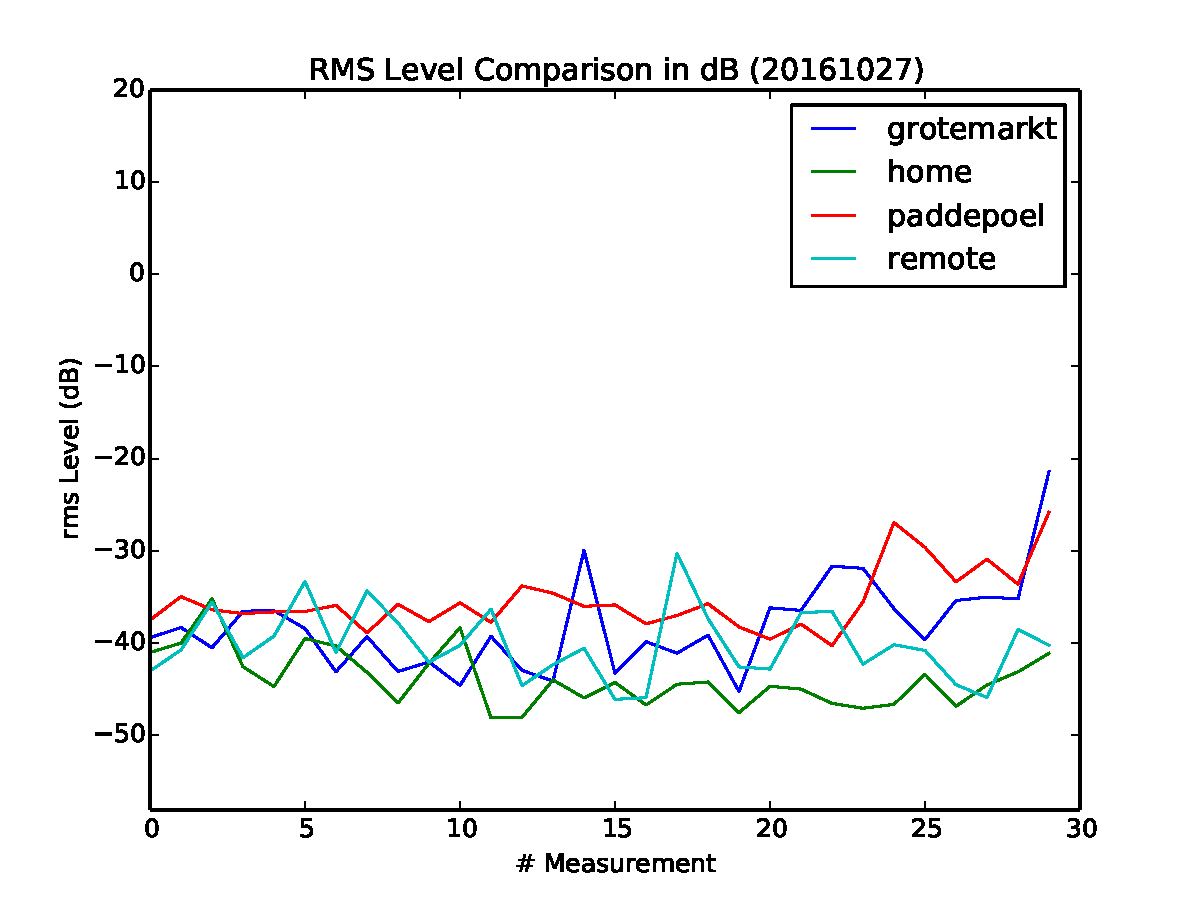
\includegraphics[width=0.7\textwidth]{./img/result/sound/rms-level-comparison20161027}
		}
	}
	\end{adjustwidth}
	\caption{Line chart showing the peak level (\ref{fig:peak-level-day2}) and root-mean-square (\ref{fig:rms-day2}) in each cycle at day 2.}
	\label{fig:audio-result-day2}
\end{figure}

\begin{table}[H]
\centering
\caption{The average of root-mean-square and peak level of ambient noise recording in day 2.}
\label{tab:ambient-noise-average-day2}
\begin{tabular}{lll} \toprule
            & \ac{RMS} (dB) & \ac{PKLV} (dB) \\ \midrule
Remote area & -40.15                & -9.53          \\
Home        & -43.89                & -18.36           \\
Paddepoel   & -35.46                & -10.51          \\
Grote markt & -38.22              & -8.33        \\ \bottomrule
\end{tabular}
\end{table}





\section{Day 3} % (fold)
\label{sec:ambient-noise-day_3}
\begin{figure}[H]
	\begin{adjustwidth}{-1cm}{}
	\centering
	\subfloat[peak level]{
		\label{fig:peak-level-day3}{
			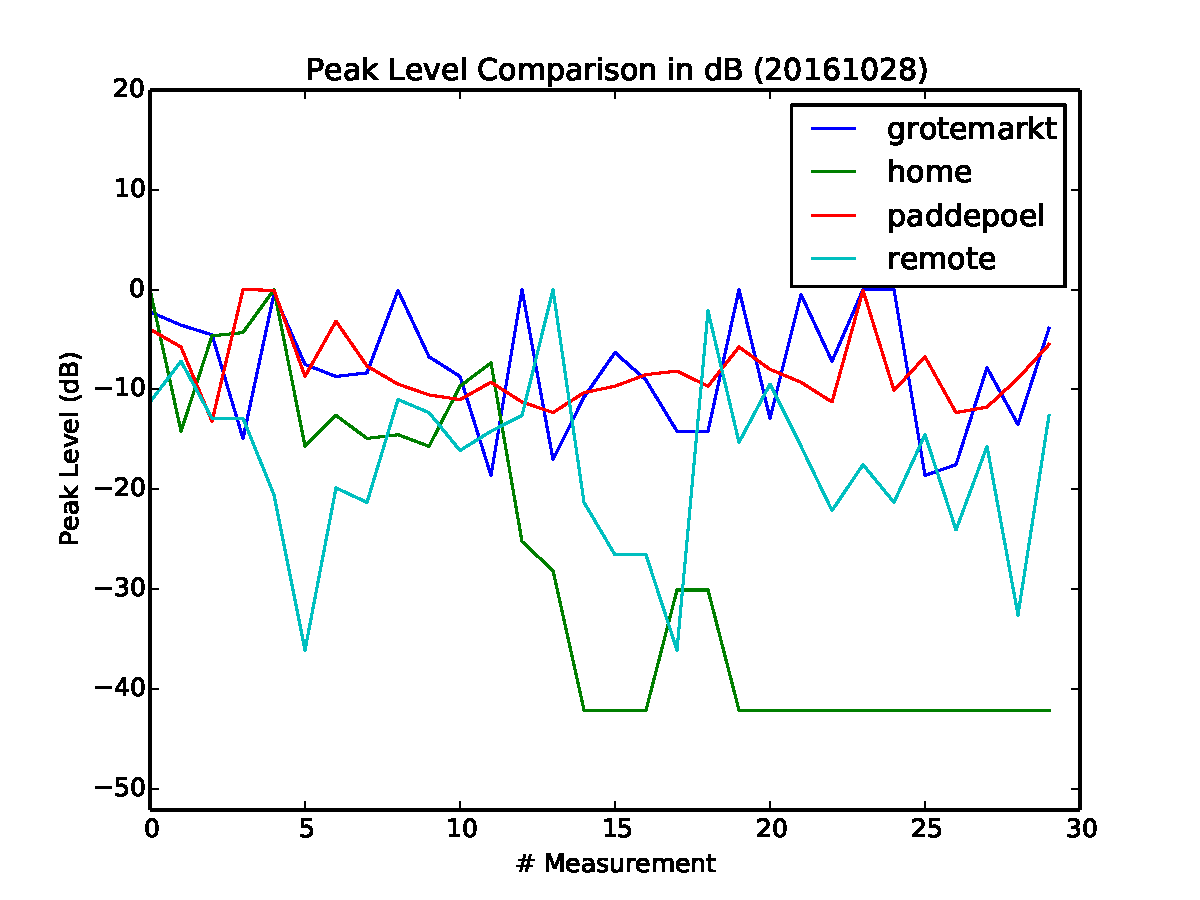
\includegraphics[width=0.7\textwidth]{./img/result/sound/peak-level-comparison-20161028}
		}
	}
	\subfloat[root mean square]{
		\label{fig:rms-day3}{
			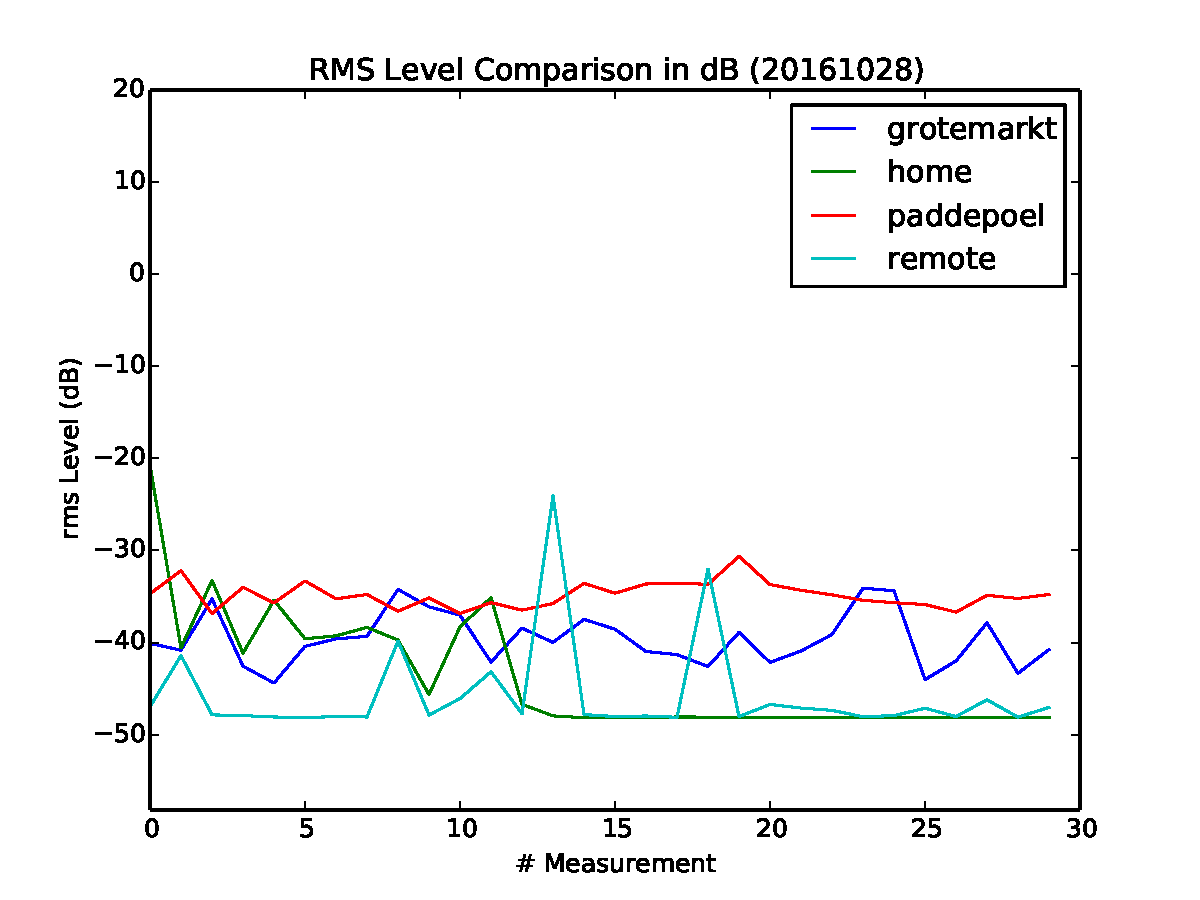
\includegraphics[width=0.7\textwidth]{./img/result/sound/rms-level-comparison20161028}
		}
	}
	\end{adjustwidth}
	\caption{Line chart showing the peak level (\ref{fig:peak-level-day3}) and root-mean-square (\ref{fig:rms-day3}) in each cycle at day 3.}
	\label{fig:audio-result-day3}
\end{figure}

\begin{table}[H]
\centering
\caption{The average of root-mean-square and peak level of ambient noise recording in day 3.}
\label{tab:ambient-noise-average-day3}
\begin{tabular}{lll} \toprule
            & \ac{RMS} (dB) & \ac{PKLV} (dB)  \\ \midrule
Remote area & -45.69                & -17.40  \\
Home        & -43.74                & -27.23  \\
Paddepoel   & -34.81                & -8.08   \\
Grote markt & -39.62              & -7.92     \\ \bottomrule
\end{tabular}
\end{table}

